\section{Optimering}
For at optimere filteret anvendes et andet vindue. Ved at eksperimentere med de forskellige vinduer ses det, at der også opstår ripples ved Blackman-vinduet, hvorimod anvendelser af Hann- og Hamming-vinduet giver ingen eller meget små ripples. Eksempler på dette er vist i figur \ref{fig:filter_Hann_Hamming}.
\begin{figure}[H]
\begin{minipage}{0.49\textwidth}
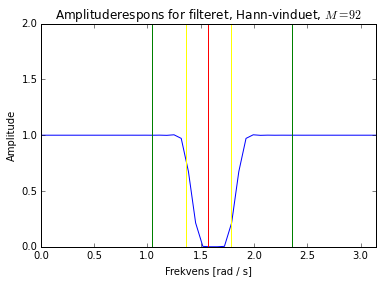
\includegraphics[width=0.9\textwidth]{figures/Filter_Hann_92.PNG}
\end{minipage}
\begin{minipage}{0.49\textwidth}
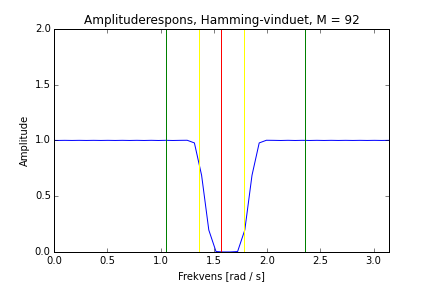
\includegraphics[width=0.9\textwidth]{figures/Filter_Hamming_92.PNG}
\end{minipage}
\caption{Eksempler på båndstopfilteret under anvendelse af Hann- og Hamming-vinduet med $M=92$.}
\label{fig:filter_Hann_Hamming}
\end{figure}

Fra figur \ref{fig:filter_Hann_Hamming} fremgår det, at der ikke er nogle ripples i pasbåndet, hvor amplituden desuden er 1. Derudover er amplituden 0 i stopbåndet, hvor $\omega_2$ ligger. Således opfylder filteret specifikationerne for denne filterorden. Lavere orden medfører færre beregninger og bredere transitionsbånd, og sidstnævnte har ikke nogen særlig betydning i dette tilfælde, fordi afstandene mellem de 3 frekvenser i signalet er så store.